\documentclass{../../Proposal/LaTeX-proposal/deliverablereport}
\usepackage{xparse}
\usepackage{etoolbox}
\usepackage{caption}
 \ExplSyntaxOn

\newenvironment{event}[6]{
\vspace{0.5cm}
\label{event-#2}

\noindent \textbf{#1}\newline % title

\noindent #3 \newline % location and date

\noindent ODK~partners~involved:~ \clist_map_inline:nn{#4}{\site{##1}~}\newline %partners

\ifx&#5&%
      % no participant #
\else
\noindent #5~participants\newline
\fi

\ifx&#6&%
      % no website
\else
\noindent \url{#6}\newline
\fi



}{\begin{center}\noindent\rule{4cm}{0.4pt}\end{center}}

 \ExplSyntaxOff


\deliverable{dissem}{workshops-1}
\issue{34}
\duedate{31/08/2016 (M12)}
\deliverydate{31/08/2106}
\author{Viviane Pons}

\begin{document}
\maketitle
\githubissuedescription

% Other tasks and deliv impacted: T3.6, T4.1, T6.1, T6.3, T6.10, D6.2

\section{Development workshops}
~

\begin{event}{OpenDreamKit Kickoff meeting}{kickoff}{Orsay (France) 2015-09-02 to 2015-09-05}{PS,UK,LL,SA,JU,UW,USH,UV,ZH,USO,US,UJF,SR}{34}{http://opendreamkit.org/2015/09/02/KickoffMeeting/}

\textbf{Main goals.} This was the starting event of the project, allowing for everyone to meet and start working.

\textbf{ODK implication.} As a lead partner, Paris-Sud was chosen to host the event. 30 ODK participants were present, 
representing most of the partners.

\textbf{Event summary.} Part of event was dedicated to ODK-specific tasks and administrative questions. But the goal
was to make much more out of it. We planned for many technical talks, presenting existing and emerging technologies
related to ODK. We also had two days of coding sprints to start working right away on ODK tasks.

\textbf{Demographic.} Most of the participants were from ODK but we had invited a few external participants.

\textbf{Results and impact.} This event set the tone for up-comming development workshops by creating a friendly, instructive, 
working atmosphere. It also set the different goals of project, allowing everyone to share their views and
understanding of ODK tasks.

\begin{figure}[ht]
\caption*{ODK Kickoff meeting}

\includegraphics[scale=0.3]{pictures/kickoff1.jpg}

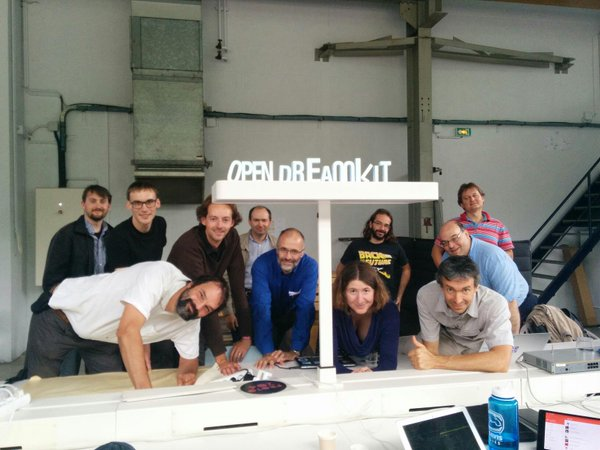
\includegraphics[scale=0.5]{pictures/kickoff2.jpg}
\end{figure}



\end{event}

\begin{event}{Sage Days 70}{sd70}{Berkeley (US California), 2015-11-08 to 2015-11-14}{PS}{16 participants}{https://wiki.sagemath.org/days70}

\textbf{Main goals.} Gather developers from Sage, SageMathCloud and Jupyter together to learn the
inner machineries of the different projects and code together towards common goals.

\textbf{ODK implication.} ODK was not the main organizer of this event, it was used to fund
European participants which are either part of ODK or very closely related.

\textbf{Event summary.} The event featured many interesting talks on the inner mechanics of
both SageMathCloud and Jupyter, in particular:
\begin{itemize}
\item \href{https://youtu.be/GOuy07Kift4}{How to contribute to SageMathCloud} by William Stein
\item \emph{The PARI Jupyter kernel} by Jeroen Demeyer
\item \emph{Jupyter Notebook development} by Jason Grout.
\end{itemize}
Lots of time was devoted to projects and code such as: installing a development version of SageMathCloud,
following tutorials on SageMathCloud development, working toward the integration of the Jupyter notebook
in Sage.


\textbf{Results and impact.} 
This workshop was essential to some ODK planned tasks. This was especially related to WP3 and WP4. Here are some tasks that
were started during the Sage Days:
\begin{itemize}
\item T3.6 Document and modularize SageMathCloud's codebase. This task was started during the workshop using the 
knowledge of the main developer of SageMathClod, William Stein.

\item T4.1 Uniform notebook interface for all interactive components. This is a major task of WP4. This workshop
was an occasion to share first hands information between Sage and Jupyter developers.
\end{itemize}
The knowledge we gathered during presentations was relevant to all tasks including notebook interfaces or cloud
systems.

\end{event}

\begin{event}{WP6 Workshop (Bremen)}{wp6-1}{Bremen, Germany, 2016-05-30 to 2016-06-03}{JU, SA, PS}{7}{}

\textbf{Main goals.} Work meeting to understand the type systems of GAP and
SAGE, and to develop a first interface between MMT, GAP, and SAGE.

\textbf{ODK implication.} Jacobs Uni Bremen was the main organizer of this
event to work on WP6.

\textbf{Event summary.} The event featured a talk about the GAP type system, and
many discussions between the researchers in Bremen and Markus Pfeiffer. We
developed a substantial piece of software to enable GAP to interface with MMT.

\textbf{Results and impact.} 
This workshop was essential to ODK WP6, in particular D6.2, T6.3.

\end{event}


\section{Dissemination and outreaching activities}

\subsection{Organization of Sage Days in established mathematical communities}
~

\begin{event}{Sage Days 74: Differential geometry and topology}{SD74}{Observatoire de Paris, Meudon, France, 30 May - 2 June 2016}{PS, UB}{26}{https://wiki.sagemath.org/days74}

\textbf{Main goals.} This workshop was dedicated to the implementation of some
topology and differential geometry in SageMath, partly in connection with the
SageManifolds project \url{http://sagemanifolds.obspm.fr/}. 3D visualisation
in the Jupyter notebook was also discussed.

\textbf{ODK implication.} ODK, via its Orsay and Bordeaux nodes, supported the travel and living expenses of 7 speakers:
\begin{itemize}
\item Marck Bell (U. Illinois, Urbana-Champaign)
\item Marck Culler (U. Illinois, Chicago)
\item Nathan Dunfield (U. Illinois, Urbana-Champaign)
\item Patrick Hooper (City College of New York)
\item Vincent Delecroix (U. Bordeaux)
\item Jeremy L. Martin (U. Kansas, Lawrence)
\item John Palmieri (U. Washington, Seattle)
\end{itemize}

\textbf{Event summary.} Morning sessions were devoted to talks on various
topics relevant to the workshop theme, some of them involving codes that are
not part of SageMath (SnapPy, Flipper, Gyoto).
Afternoon sessions were devoted to working groups and coding sprints.

\textbf{Demographic.}
26 persons took part in these Sage Days: 5 females and 21 males, originating
from the following countries: France (11), USA (8), Poland (3), Germany (2), Russia (1) and UK (1).


\textbf{Results and impact.}
41 SageMath tickets have been written or reviewed during the workshop; the list
of them is available at \url{https://trac.sagemath.org/query?keywords=~sd74&or&keywords=~days74}
Progresses on the K3D-jupyter visualisation are reported at
\url{https://wiki.sagemath.org/K3D-tools}.

\end{event}


\begin{event}{Sage Days 78}{sd78}{Vancouver (Canada), 2016-06-29 to 2016-07-01}{PS, UB}{30}{https://wiki.sagemath.org/days78}

\textbf{Main goals.} The event was organized as a satellite event of the yearly international conference
in algebraic combinatorics \href{https://sites.google.com/site/fpsac2016/}{FPSAC}. The objective was to gather
the combinatorics community around Sage development, to introduce Sage to newcomers (especially graduate students) and
to bring new Sage contributions.

\textbf{ODK implication.} the event was co-organized by ODK (trough Viviane Pons) and the 
\href{https://www.pims.math.ca/}{Pacific Institute for the Mathematical Science} where
it was hosted. The event costed around 4000 CAD (2000 CAD from ODK).
 A short presentation about ODK was made during the conference to present 
the project to the participants.

\textbf{Event summary.} We started the event by some introduction presentations and tutorials so that
the participants would familiarized themselves with Sage. Then the time was shared between lectures
and coding sprints. Here are some highlights:
\begin{itemize}
\item Our invited speaker \textbf{Mike Zabrocki} (York Univ.) gave a lecture on \emph{Open Problems in Combinatorial Representation Theory}.

\item \textbf{Emily Gunawan} (Univ. of Minnesota) and \textbf{Jessica Striker} (North Dakota State Univ.) gave respectively
a tutorial and a lecture on \emph{Research-based coding} for Sage.

\item An undergrad student \textbf{Amit Jamadagni} gave a presentation of the extensive package on \emph{Knot Theory} that
he developed during a Google Summer of code project.
\end{itemize}

The full program can be found on the website \url{https://wiki.sagemath.org/days78}. We planned lots of time for 
participants to work on development projects such as: Plane partitions, plotting functions for combinatorics
objects, Lie algebras, Rook replacement...

\textbf{Demographic.} The participants were required to fill out a demographic survey. We had 29 participants (24 males and
5 females), 27 identified as academics: 7 professors, 6 postdoc, 11 graduate students, and 3 undergrads. 19 participants
were from North America (10 from Canada and 9 from the US), 8 were from Europe (France, Austria, and Switzerland), and 3 from 
Asia (South Korea and India).

\textbf{Results and impact.} 
\begin{itemize}
\item \textbf{New comers got to use Sage for the first time} around one
third of the participants had zero or very little experience with Sage before the meeting. By the
end of the three days, everyone had a way to use Sage (either online or on their machines)
and had written a bit of code.
\item \textbf{New comers got to contribute to Sage}: a lecture was given on how to contribute to Sage
and groups were formed on different projects mixing more experienced people with new comers so
that the code that was written could end up being merged to the software. In particular, a implementation
of Plane Partitions was put together by a participant who had never used Sage before.
\item \textbf{New contributions were made in the combinatorics component of Sage}: we used the keyword
\textbf{days78} on the trac server of Sage to track the contributions that were submitted during the workshop.
 Altogether the participants
worked on 17 different tickets either reviewing
existing ticket, implementing, or creating new tickets. 6 of them already got positive reviews and are
on the process of being merged to the software.
\end{itemize}

\begin{figure}[ht]
\caption*{Participants of Sage Days 78 making Sage demo}
\begin{tabular}{cc}
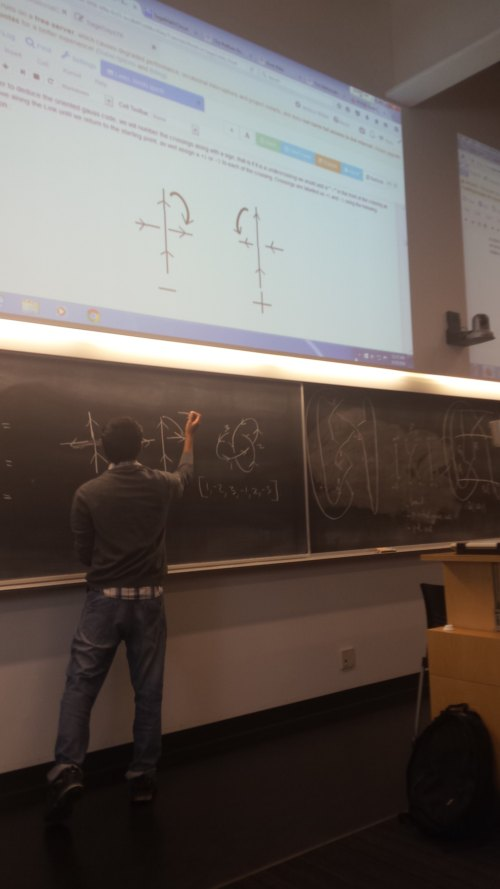
\includegraphics[scale=0.3]{pictures/sd78-1.jpg}
&
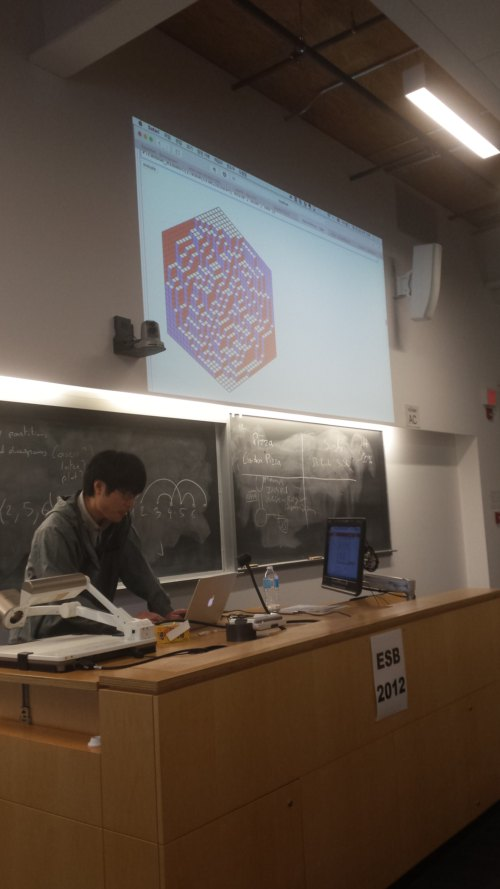
\includegraphics[scale=0.3]{pictures/sd78-2.jpg}
\end{tabular}
\end{figure}



\end{event}

\subsection{Fostering a community in North Africa and Mediterranean countries}

\subsection{Other training activities}

\subsection{Communication and participation to external events}
~


\begin{event}{PyConFr}{pyconfr}{Pau (France), 2015-10-17 to 2015-10-18}{PS}{around 200 participants}{http://www.pycon.fr/2015/}

\textbf{Main goals.} PyConFr is the main gathering of the python community in France. It is a good place to meet the 
French open source python community and to talk and learn about projects.

\textbf{ODK implication.} Viviane Pons was present at the meeting and she gave a talk
on her \href{http://www.pycon.fr/2015/schedule/presentation/16/}{teaching experience using SageMathCloud}. She was
also part of a panel on diversity. 

\textbf{Results and impact.} This event was an occasion to introduce ODK to the larger python community in France as well as to
keep active the link between Sage development and other python open source projects. It is always a great occasion to discuss subjects
 such as user interfaces, cloud servers, best practices, communities, etc. The diversity panel in particular was a great success bringing
 together most of participants of the event. As this is a great concern for ODK, we were happy to be part of it.


\end{event}

\begin{event}{Finite Simple Groups: Thirty Years of the Atlas and
    Beyond}{tyatlas}{Princeton (US California), 2015-11-02 to 2015-11-05}{PS}{94
    }{http://math.arizona.edu/~grouptheory/princeton/}

\textbf{Main goals.} Gather contributors to and users of the ``Atlas of Finite
Simple Groups'' and other mathematical databases to learn about past, presence,
and future.

\textbf{ODK implication.} ODK was not the main organizer of this event, it was used to fund
a European participant.

\textbf{Event summary.} The event featured talks by high-profile mathematicians,
such as John H. Conway, John Thompson, Michael Aschbacher, and many more.

Discussion sessions highlighted the need for mathematical knowledge
stored in databases. Some major examples that were discussed are
\begin{itemize}
  \item The ``ATLAS of Finite Group Representations - Version 3''
    http://brauer.maths.qmul.ac.uk/Atlas/v3/
  \item The ``Online Encyclopedia of Integer Sequences (OEIS)''
    http://oeis.org
  \item The ``Modular forms and L-functions database (LMFDB)''
    http://lmfdb.org
  \item The ``Small Groups Database'' (small)
\end{itemize}

Most of these databases share common issues such as \emph{reliability} of the
data, the \emph{reliability} and \emph{longevity} of the storage,
\emph{maintenance}, and \emph{managing contributions}.
    
\textbf{Results and impact.} 
The attendance of this conference shed light on how some mathematicians view
mathematical databases, and what issues they see. This is an important
contribution for WP6. It also contributed to the attendee's understanding of the
needs of our potential users (WP4).

\begin{itemize}
\item T6.1 Survey of existing DKS bases, Formulation of Requirements
\item T6.10 Math Search Engine

\end{itemize}

Further discussions with GAP users and developers about HPC-GAP were a
side-effect of the attendance of this event. 

\end{event}

\begin{event}{13th Joint Magnetism and Magnetic Materials (MMM) -
    Intermag Conference}{mmm2016}{San Diego (CA, USA), 2016-01-11 to
    2016-01-15}{USO}{30}{https://magnetism.org}

  \textbf{Main goals.} The main goals of presenting the project at
  this important international Joint Magnetism and Magnetic Materials
  and Intermag conference was to introduce the Micromagnetic Virtual
  Reasearch Environment (VRE) to our target user audience - the
  micromagnetic scientific community.


\textbf{ODK implication.} The OpenDreamKit project has sent the
speaker (Hans Fangohr), and paid expenses for the trip.

\textbf{Event summary.} Hans Fangohr submitted a talk \cite{16FangohrOOMMF} that was peer
reviewed and accepted for presentation. In the talk, he outlined the
vision for the project and invited feedback from the community.

The ODK project for computational micromagnetics was discussed with
various attendees informally throughout the conference.

In addition, we organised a meeting with the main developers of the
OOMMF micromagnetic simulation code, Dr M. Donahue and
Dr D. Porter, in order to discuss the project's vision, our plans for
interfaces to get early feedback.


\textbf{Results and impact.} We announced the project and its website
to the community and encouraged input to extend our vision, to make
sure the tool we develop can be as practical and efficient for as
large parts of the community as possible.

\end{event}


\begin{event}{First Joint GAP-SageMath Days}{GAPSage2016}{St Andrews (UK),
2016-01-18 to 2016-01-22}{USTAN,UPSud,UVSQ,UNIKL,UOXF)}{19}{http://gapdays.de/gap-sage-days2016/}

\textbf{Main goals.}

Both GAP and SageMath systems have traditions of regular developer meetings, where those
interested in these systems, from newcomers to contributors, are gathering together for
collaborative code writing, sharing best practices, advertising recent new features and
improvements, and discussing further developments. You can find the list of previous GAP 
days at \url{http://gapdays.de/} and of SageMath days at \url{https://wiki.sagemath.org/Workshops}.

Following these traditions, it was decided to organise the 1st Joint GAP-SageMath Days, with the
focus on improving GAP-SageMath integration and interaction between these systems and between
their developers.

\textbf{ODK implication.} 
%Describe how ODK was involved and give a rough estimation of cost for ODK

The 1st Joint GAP-SageMath Days were mainly supported by CoDiMa -- Collaborative Computational
Project (CCP) in the area of Computational Discrete Mathematics (EPSRC grant EP/M022641/1,
\url{http://www.codima.ac.uk/}). It was immediately followed by the WP7 Workshop ``Knowledge
representation in mathematical software and databases'' on January 25th-27th, 2016, therefore
OpenDreamKit participants involved in GAP and/or SageMath development could conveniently attend
both events. Accommodation, subsistence and travel expenses of partners from UPSud and UVSQ
were paid by the OpenDreamKit project, and those of partners from UNIKL,UOXF were reimbursed
by the CoDiMa project.

\textbf{Event summary.} 
%Give a summary of your event

A typical day of the workshop had one or two introductory talks to facilitate subsequent
discussions and coding sprints, in particular:
\begin{itemize}
\item \emph{Contributing to Sage} by Nicolas Thiery and Volker Braun
\item \emph{Contributing to GAP } by Max Horn, Alex Konovalov and Markus Pfeiffer
\item \emph{libGAP} by Volker Braun
\item \emph{GAP in the cloud} by Markus Pfeiffer
\end{itemize}
Other topics included, among others,
further integration of HPC-GAP into GAP;
working on the semantic-aware SageMath interface to GAP;
improving the installation of GAP in SageMath and in SageMath cloud;
creating and working with Docker containers;
development of GAP and SageMath teaching materials for Software Carpentry,
etc.

\textbf{Results and impact.} 
% What did you achieve with this event? (If ever it impacted 
% other ODK tasks and deliverables, mention it here)

The workshop was very productive. Only to the main GAP repository 
(\url{https://github.com/gap-system/gap/) there were 51 new pull 
requests submitted, just 8 of which are still open; in addition,
28 new issues were created (9 of them are closed by now), and 
there was also progress achieved with GAP packages developed 
elsewhere; the work on converging GAP and HPC-GAP; discussing 
development workflows, etc. It helped to both GAP and SageMath 
teams to get further insights into each other's systems and was 
particularly beneficial to WP3 (component architecture), WP4 
(user interfaces) and WP5 (high-performance computing). 

\end{event}

\begin{event}{International Workshop on Software Engineering for
    Science}{se4science2016}{Austin (TX, USA),
    2016-05-16}{SOUTHAMPTON}{15}{http://se4science.org/workshops/se4science16/}

  \textbf{Main goals.} Spread recommendations to support better
  science in the area of software engineering for computational research.

  \textbf{ODK implication.} The work presented has been created with
  the upcoming Jupyter OOMMF integration in mind, and is of wider
  interest to the OpenDreamKit partners and users. The conference
  attendance was paid from a different grant.

  \textbf{Event summary.} Hans Fangohr delivered a talk on Software
  Engineering for Computational Science, in particular reviewing
  technical and social aspects of a computational science code that
  was developed about 10 years ago. The presentation [1], and associated
  publication [2] extracted lessons learned from the past and with the aim
  to enable the community to identify potential mistakes sooner. The
  presentation and work provides recommendations to enable better
  science in the field of computational science and engineering; in
  particular focusing on software engineering for computational
  science and research codes.

  The talk was the keynote presentation of the morning session in the
  workshop on Software Engineering for Science (30 minutes).

  \textbf{Demographic.} About 15 people were present, 3 female.

  \textbf{Results and impact.} We reported evidence from the
  effectiveness of particular sofware engineering techniques and
  provided recommendations for future projects (including user
  interface, testing, version control, documentation,
  installation).

  [1]
  \href{http://www.southampton.ac.uk/~fangohr/publications/talk/2016-05-16-ICSE-SE4Science-Austin-Texas-US.pdf}
  {slides as pdf}

  [2] Hans Fangohr etal, ``Maximilian Albert and Matteo Franchin Nmag
  micromagnetic simulation tool - software engineering lessons
  learned'', Proceedings of the International Workshop on Software
  Engineering for Science, at ICSE2016 SE4Science '16, Austin, Texas,
  US, 1-7 (2016)


\end{event}


\begin{event}{PyCon}{pycon}{Portland (Oregon), 2016-05-28 to 2016-06-02}{PS}{around 3000}{https://us.pycon.org/2016/}

\textbf{Main goals.} PyCon is the biggest python conference in the world. It is the best place to learn
about the python community, open-source tools, new technologies, etc. It is also a good place
to grow a network in the software development community.

\textbf{ODK implication.} Viviane Pons was present at the meeting for the third time in a row,
consolidating her effort to build links between Sage and python communities. In 2015, she had given
a talk and organized a parallel Sage Days event. It was not possible to do so this year but a
Sage sprint was still maintained.

\textbf{Results and impact.} The conference itself was very instructive as usual in thematics such as:
efficient programming, parallel computing, open-source community building, teaching, inclusivity. It
was a good occasion to discuss with other python programmers and introduce the ODK project. The academic
community did not seem as present as it had been in the previous years. In the future, we might want to
target smaller events such as SciPy and EuroScipy.
\end{event}

\begin{event}{5th Encuentro Colombiano de Combinatoria}{ecco}{Medellin (Colombia), 2016-06-13 to 2016-06-24}{PS}{130}{http://ecco2016.combinatoria.co/}

\textbf{Main goals.} ECCO is a combinatorics summer school organized every other years in Colombia. It welcomes 
students from all over the world of all levels: from undergrad to postdocs. It is known to be a very
interesting event and has a great impact for combinatorics in Colombia and South America in general.
The Sage community in combinatorics being very active, it was a great occasion to introduce Sage
to a new generation of researchers.

\textbf{ODK implication.} Viviane Pons was sent by ODK to give two Sage interventions
during the school.

\textbf{Event summary.} Each intervention was 2 hours long with around 50 participants each time.
Most participants were using the university computers. 50 usb sticks were bought previous
to the conference and set up with bootable Linux and sage, allowing for a very quick setup
during the two sessions without relying on on-line options. The students worked on some
introduction tutorials and also specifically made tutorials in relation with the on-going
classes.  

\textbf{Demographic.} 66 participants came from South and Central America, 34 from North America
and 30 from Europe. 

\textbf{Results and impact.} 
\begin{itemize}
\item The organizers were very happy that ODK would propose to send someone at the school. 
They did not have anyone who could carry such an intervention which requires both Sage and
technical skills.

\item It was quite a challenge to get Sage to work in approximatively 10 minutes for 50
computers all together. The solution of the bootable USB key has been developed by Thierry
Monteil but is not well known nor well documented. This was an occasion to test this solution
in this particular setup and improve our experience for future events.

\item The bootable USB keys were very successful and many students brought their own keys to
get a copy of the software. During the sessions, we could also help students install
Sage on their own computers.

\item Many of the students, especially the younger ones from South America, had never used
Sage before. We proposed many different tutorials so that everyone could have something to
work on and we created exercises related to the class content of the two weeks. We received
 enthusiastic feedbacks for the sessions.

\item Some of the introduction tutorials of the Sage documentation were translated into 
Spanish for the sessions and will eventually be added to Sage.

\item The conference in general was a very rewarding event. It has been growing and successful
for the past ten years with a strong focus on inclusivity and impact. It was a great occasion
to be part of the event and learn from their experience. A blog post from Viviane Pons was
published by the \emph{AMS Blog on Teaching and learning mathematics} [CITE HERE].
\end{itemize}



\begin{figure}[ht]
\caption*{Participants of ECCO at the Sage sessions}
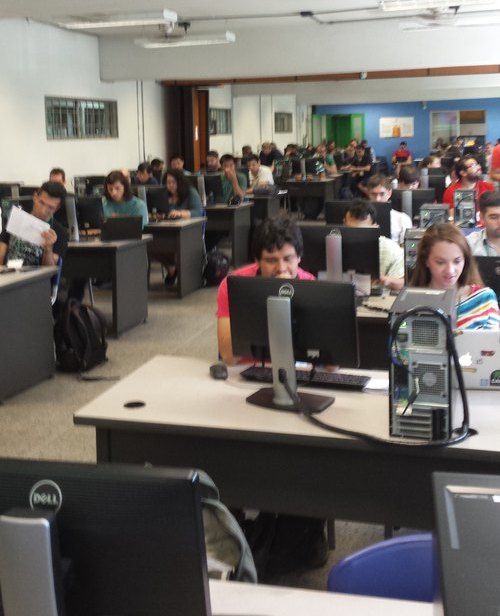
\includegraphics[scale=0.5]{pictures/ECCO-1.jpg}

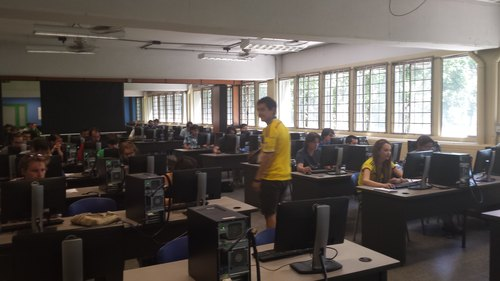
\includegraphics[scale=0.5]{pictures/ECCO-2.jpg}
\end{figure}



\end{event}

\begin{event}{Invited Seminar Talk at ``Universidade Nova de
    Lisboa''}{lisbon}{Lisbon, Portugal), 2016-07-19}{USO}{6 participants}{}

\textbf{Main goals.} Advertise capabilities of OpenDreamKit with a research talk
that showcases the GAP Jupyter interface.

\textbf{ODK implication.} Markus Pfeiffer showcased the GAP Jupyter notebook
interface as part of a research seminar talk on search in permutation groups.

\textbf{Results and impact.} 
This seminar talk was a good opportunity to advertise OpenDreamKit outside of
our core developer- or usergroups.

\end{event}



\section{Upcoming events and plans for the future}

\bibliographystyle{plain}
\bibliography{report}

\footnotesize{All referenced ODK talks are available as annexes}
\end{document}

%%% Local Variables:
%%% mode: latex
%%% TeX-master: t
%%% End:
